In this chapter, we discuss the transition scenarios for new nuclear reactor deployment in the \gls{usa} and the reactor models used in this work. We also discuss the theoretical framework and key concepts that underpin the research and the results for each deployment scheme.

\section{Transition Scenarios}
\label{sec:transition_scenarios}
% Discuss the theoretical framework and key concepts that underpin the research.

As the energy landscape evolves, compounding factors will drive the actual deployment of these reactors in ways this work does not capture. The value of energy system modeling and transition scenarios is to understand the deployment implications compared with and measured relative to business-as-usual cases with similar approximations.

We use this chapter to explore the deployment schemes we have
implemented---outlined in Table \ref{tab:deployment_schemes}---and the demand
growth scenarios we have considered---outlined in Table
\ref{tab:demand_scenarios}. In Appendix \ref{sec:considered_deployment_schemes}
we will discuss two additional deployment schemes that we implemented but
have not incorporated, as they are more useful for problems not considered herein.

\begin{table}[H]
    \centering
    \caption{Deployment schemes.}
    \label{tab:deployment_schemes}
    \begin{tabular}{p{0.15\linewidth} >{\raggedright}p{0.20\linewidth}>{\raggedright\arraybackslash}p{0.50\linewidth}}
        \hline
        Status & Scheme & Description \\
        \hline
         & Greedy Deployment & Deploy the largest
        reactor first at each time step, fill in the remaining capacity with
        the next smallest, and so on. \\
        Incorporated & Random Deployment & Uses a date and hour as seed to sample the
        reactors list randomly. \\
        & Initially Random, Greedy Deployment & Randomly deploy reactors until
        a reactor bigger than the remaining capacity is proposed for each time step,
        then fills the remaining capacity with the greedy algorithm. \\
        % & Single Reactor & A single reactor model is deployed as the existing fleet is decommissioned.\\
        \hline
         & Capped Deployment & There is a
        single-number capacity for one or more of the reactor models. \\
        Not Incorporated & Pre-Determined Distribution Deployment & One or more reactors have a
        preset distribution, and a smaller capacity model fills in the gaps. \\
        \hline
    \end{tabular}
\end{table}

We apply these deployment schemes to demand growth scenarios based on two
predictions of future energy demand. The \gls{eia} publishes demand expansion
projections for the totality of the \gls{usa} \cite{eia_aeo_2023}. The
administration has refrained from publishing AEO 2024 in light of recent
accelerations in demand growth. Our assumptions for the low-growth scenarios
are that the relative percentage of nuclear power remains constant and that the
relative performance of the various fuel cycle metrics we simulate will remain
constant. Our high-growth scenarios come from the \gls{doe} Liftoff Report
\cite{julie_liftoff_pathways_2024}, which does not reflect this constant
percentage assumption for nuclear power in their demand scenarios. Their growth
projections are specific to nuclear energy deployment increases, and the number is agnostic to the total increase.

\begin{table}[H]
    \centering
    \caption{Demand growth scenarios.}
    \label{tab:demand_scenarios}
    \begin{tabular}{l c c}
        \hline
        \textbf{Demand Growth} & \textbf{Year-to-Year Increase} & \textbf{Source}\\
        \hline
        No Growth & 0\% & N/A\\
        Low Growth & 0.17\% & \cite{eia_aeo_2023}\\
         & 0.5\% & \cite{eia_aeo_2023}\\
         & 1\% & \cite{eia_aeo_2023}\\
        High Growth & 3.5\% & \cite{julie_liftoff_pathways_2024} \\
         & 5.6\% & \cite{julie_liftoff_pathways_2024}\\
        \hline
    \end{tabular}
  \end{table}

Each growth scenario is deployed under two regimes: 1) the reactors are never
fueled with \gls{leup}; 2) the \gls{mmr} and \gls{xe} reactors are fueled with
\gls{leup} until 2040, when they move to \gls{haleu}. \glspl{mmr} deployed
before this fuel transition will continue to use \gls{leup} fuel until the end
of their lifetime as they do not refuel; however, the \gls{xe} reactors will
refuel with \gls{leup} until 2040, when they will refuel with \gls{haleu}. The
AP1000 reactors will continue to use \gls{leu} fuel throughout the simulation.

Under a regime, each growth scenario is met by deploying reactors using the
schemes outlined in Table \ref{tab:deployment_schemes}. We will discuss the
results of these deployment schemes in the following sections. We will also
discuss the limitations of this work and propose future work. Regardless of the
regime, each deployment scheme will attempt to deploy reactors to meet the
capacity outlined in Figure \ref{fig:dep_goals}. We will focus on the results
of the no growth and $3.5\%$ (corresponding to doubling nuclear by 2050)
scenarios.

\begin{figure}[H]
    \centering
    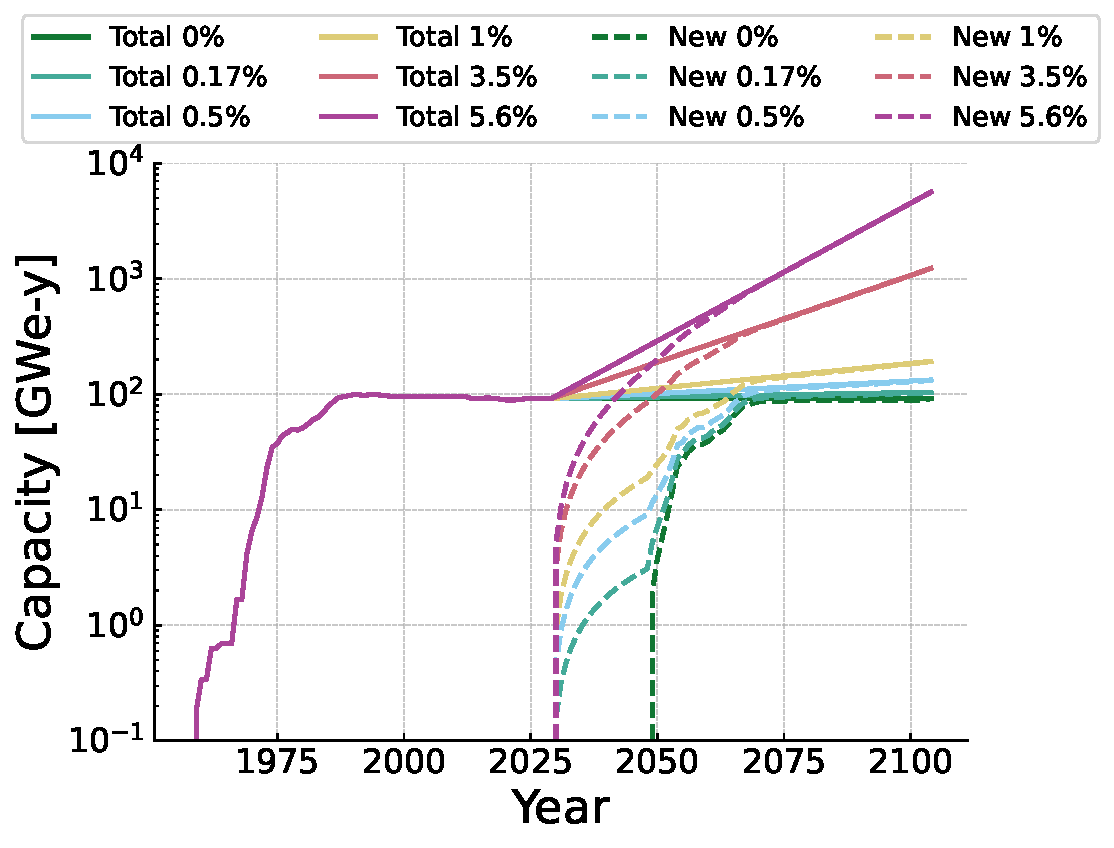
\includegraphics[scale=0.7]{images/results/deployment_calcs/total_new_capacity_scenarios.pdf}
    \caption{Total and new nuclear capacity deployed in each scenario.}
    \label{fig:dep_goals}
\end{figure}

As shown, advanced reactors (for this work, the designs are the \gls{mmr},
\gls{xe}, and AP1000) begin deployment in 2030. While this is an aggressive deployment schedule, \cite{bachmann_thesis_2023} established that the precise deployment start did not significantly impact the total results for this type of analysis and could reasonably serve as an upper bound of deployment. The business-as-usual or, as we will refer to it, no growth scenario does not require the deployment of a new nuclear reactor until just before 2050, whereas the other scenarios understandably commence deployment in 2030. As we have presented the capacity on a logarithmic plot, the linear appearance of the data belies the compounding effect that the year-to-year percentage growth requires.

Comparing these projected deployments with the results from the no growth and double scenarios, we can consolidate the over and under deployments of capacity into Table \ref{tab:cap_diff} and see that the random deployment scheme showed the least total difference between the results and the projection. The initially random, then greedy deployment scheme showed the largest total difference between the results and the projection, while the greedy deployment scheme was between the two.

\begin{table}[H]
    \centering
    \caption{Capacity difference between results and projection.}
    \label{tab:cap_diff}
    \begin{tabular}{c c c}
        \hline
        Scenario & Deployment Scheme & Total Difference [GWe]\\
        \hline
        \multirow{3}{*}{No Growth} & Greedy & 19.46 \\
        & Random & -15.21 \\
        & Initially Random, Greedy & 47.26 \\
        \hline
        \multirow{3}{*}{Double} & Greedy & 103.54 \\
        & Random & 6.65 \\
        & Initially Random, Greedy & 151.86 \\
        \hline
    \end{tabular}
\end{table}

We show the difference in energy output between the results and the projection for the no growth and double scenarios over time in Figure \ref{fig:e_diff}. The difference curves in Figure \ref{fig:e_diff_d2} show a tightly perturbed oscillation as more reactors are deployed to meet the increasing demand in the random and the initially random, then greedy schemes. Closer to the start of advanced reactor deployment, the greedy scheme shows a consistently smaller difference than the other schemes, but the difference continues to grow as time progresses.

\begin{figure}[H]
    \subfloat[No Growth. \label{fig:e_diff_ng}]{%
      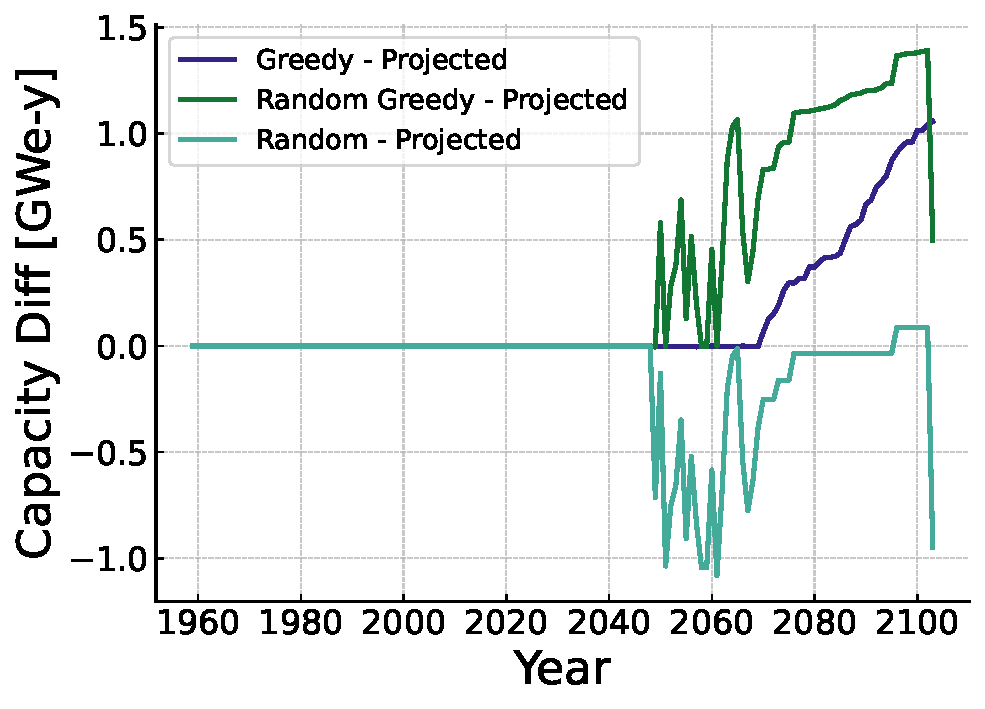
\includegraphics[width=0.495\textwidth]{images/results/energy/ng_diff.pdf}
   }
    \hfill
    \subfloat[Double. \label{fig:e_diff_d2}]{%
      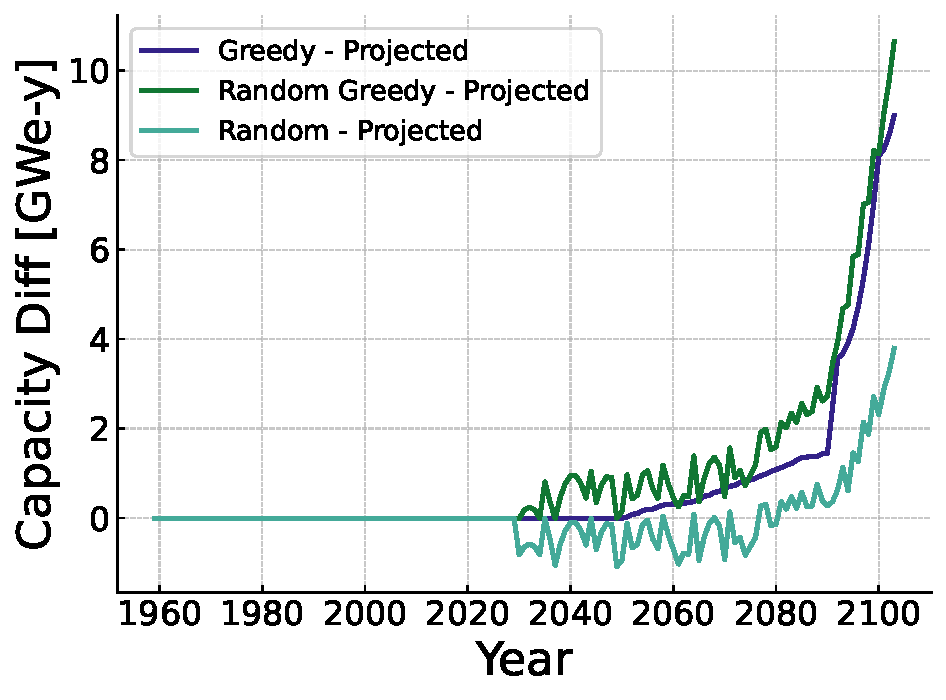
\includegraphics[width=0.495\textwidth]{images/results/energy/d2_diff.pdf}
   }
    \caption{Energy output difference between results and projection.}
    \label{fig:e_diff}
\end{figure}

